\begin{figure}
\centering 

\subfigure[Pressing a mouse button exerts force perpendicular to the
  operating plane.] { 
  \label{fig:button-force-mouse} 
  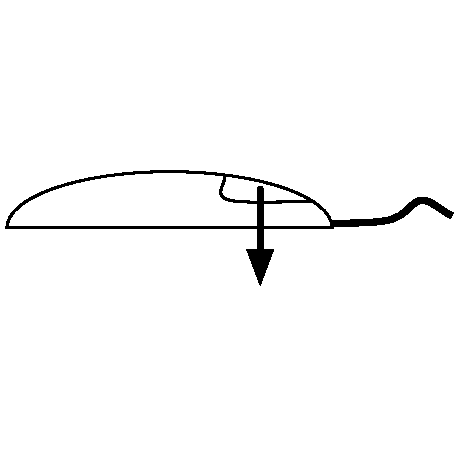
\includegraphics[origin=c, width=5.5cm]{img/button-force-mouse.pdf} 
}
\hspace{1cm} \subfigure[Pressing a stylus button is likely to cause
  accidental pen tip movement.] {
    \label{fig:button-force-pen}
    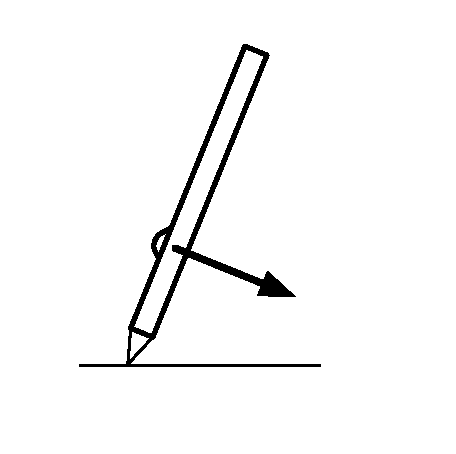
\includegraphics[origin=c, width=5.5cm]{img/button-force-pen.pdf}
}
\caption[Pen vs. Mouse]{The force required to press a mouse button compared with a
  stylus button.}
\label{fig:button-force}
\end{figure}
